\documentclass[pdflatex,sn-vancouver-num]{sn-jnl}
\usepackage{graphicx,booktabs,array,longtable,amsmath,xcolor,needspace}
\raggedbottom\hypersetup{hidelinks}
\renewcommand{\thesection}{S\arabic{section}}\renewcommand{\thetable}{S\arabic{table}}\renewcommand{\thefigure}{S\arabic{figure}}
\begin{document}
\title[Supplementary information]{Additional file 1: Supplementary methods and results}
\author[1]{\fnm{Author names} \sur{to complete}}
\affil[1]{\orgname{Institution to complete},\orgaddress{\country{China}}}
\abstract{This supplement provides source and endpoint definitions, model specifications, complete supporting results, and additional figures for the cross-setting evaluation of recorded-anemia prediction after acute myocardial infarction.}
\maketitle
\section{Source handling and endpoint implementation}

The local diagnosis-triggered source files were retained unchanged and checked for internal consistency. Worksheet dimensions, identifiers, and duplicate admission records were independently inspected. Admissions shared with the linked historical coronary export agreed on demographic and admission information, and 31,915 overlapping laboratory keys matched on patient, admission, test, time, and displayed result. These checks supported linkage integrity but did not establish complete hospital-wide capture or independent clinical adjudication.

The diagnosis-triggered export selected patients with a primary or secondary AMI discharge diagnosis and included other admissions belonging to those patients. Primary-ACS index-admission selection and restriction to primary AMI were applied subsequently. Earlier visible ACS admissions from a linked historical coronary export were considered before Hb eligibility; the historical export's treatment-based selection criteria were not imposed on the principal cohort. Diagnoses were derived from discharge records without further study-specific clinical adjudication. Admission-level procedure assignment used records with patient and admission identifiers; unlinked procedure entries were not treated as admission-specific evidence.

Early Hb normality required every valid D0--1 measurement to meet the sex-specific threshold, whereas the most recent early daily median was used for prediction. Displayed laboratory results, rather than automatically substituted machine-numeric values, determined eligibility and outcomes. Uninterpretable or inequality-coded results, incompatible specimens, and implausible values were handled using documented harmonization rules. Observation-day counts reflected distinct D0--1 calendar days, not repeated draws within a day. Laboratory standards and limits are given in Table~\ref{tab:s2}; the feature dictionary and detailed implementation are provided in the repository described in the main manuscript.

The prediction landmark was the beginning of calendar D2. Because local discharge timestamps were not available, admissions discharged on D2 were excluded, including two otherwise early-normal stays. Future Hb observation on D2--7 defined whether the conditional recorded-anemia endpoint could be evaluated; absence of future Hb was not assigned a negative conditional label. Alternative follow-up windows retained only patients with observable outcomes in the relevant window. The daily-median and last-day endpoints were derived from available future results. Signed Hb decline was calculated as the first early daily-median Hb minus the recorded future minimum and could be negative. Missing-label completion scenarios do not estimate unmeasured biological anemia.

\section{Model freezing, supporting experiments, and evidence limits}

All conditional models, alternative observation representations, observation models, Ridge regressions, and public-development sensitivity models were fitted and calibrated using public data. Their saved preprocessing, fitted parameters, and calibration transformations were applied unchanged in local evaluation. The candidate observation representations were examined post hoc, informed by earlier local findings; local labels were not used to fit or calibrate the frozen public models. Analyses and code provenance are documented in the accompanying repository.

M0--M3 used public-training median imputation, standardization, and logistic regression ($C=1$). M4 used the M2 inputs and histogram gradient boosting (150 iterations; learning rate 0.05; 7 leaves and L2 regularization of 10 selected by public-training cross-validation). A separate public calibration set supported logistic transformation of predicted log-odds. M1D added early Hb change to M1. A1 added missingness indicators alone to M2; A2 added observation-day counts alone. A3 removed albumin concentration from M2; A4 removed only the albumin observation inputs from M3; A5 removed albumin concentration from M4; and A6 removed albumin concentration and its observation inputs from M3. B1 and B2 combined M2 physiological inputs with at-least-one-day and at-least-two-day observation indicators, respectively, without separate missingness flags.

Observation models O1--O3 predicted future Hb availability, and J1--J3 were the products of the corresponding frozen observation and conditional-anemia probabilities without further recalibration. Ridge models used $\alpha=1$ and a public-calibration mean-residual correction. Source classification used five stratified folds and predicted dataset origin, not anemia. Local intercept-only and intercept-and-slope updating used ten repeated five-fold partitions, with out-of-fold evaluation; repetition ranges describe split variability rather than confidence intervals or independent validation.

Observation-weighted analyses used the frozen public O3 probabilities with lower clipping at 0.05 or 0.10. Neither missing-at-random assumptions nor transport of the observation model was established. In 200 retained-record simulations, one future Hb result per patient per calendar day was sampled before rebuilding observed outcomes; this did not simulate unrecorded blood draws. Fixed-model intervals used 1,000 patient-level bootstrap draws paired across models, excluding single-class resamples from AUROC estimation. Separate public-development analyses comprised 300 bootstrap repetitions and 20 repeated splits; they did not quantify full development uncertainty in the local evaluation.

Local procedure dates were available at day precision, with incomplete operative-note coverage. Positive procedure-name or transfusion evidence was used descriptively; absent records were not interpreted as verified treatment absence. Graft angiography was not classified as new CABG, and transfusion-reaction codes alone were not considered evidence of transfusion. Available fields did not support exact elapsed-48-hour, medication-dose, or transfusion-timing analyses. No clinical intervention or decision threshold was validated.

Model-evaluation software included Python 3.12, scikit-learn 1.4.2, and pandas 2.2.2. The primary development, exploratory development, and local evaluation seeds were 20261014, 20261015, and 20261022, respectively. Source extraction and model evaluation used separate documented runtimes, with intermediate files used only for private analysis.

\section{Supplementary tables}
\begingroup\scriptsize\setlength{\tabcolsep}{2pt}
\begin{longtable}{p{8.5cm}r}
\caption{Local export and cohort flow}\label{tab:s1}\\
\toprule
Stage & N\\\midrule
\endfirsthead
\toprule
Stage & N\\\midrule
\endhead
\endfoot
\bottomrule\endlastfoot
Exported stays & 436\\
Exported people & 399\\
Primary AMI stays & 320\\
First visible ACS is AMI (diagnosis-triggered export) & 306\\
Strictly beyond D2 discharge-date boundary (pre-reconciliation) & 287\\
Primary-AMI index patients after linked history and conflict review & 280\\
Early normal before linked-history reconciliation & 118\\
Early normal after linked prior-ACS history review & 116\\
Future Hb observed & 100\\
Recorded anemia & 46\\
No recorded anemia among observed & 54\\
Future Hb unknown & 16\\
\end{longtable}
\noindent\textit{Note:} The initial export and history-reconciled counts represent related but not strictly sequential selection stages. After linked-history, primary-diagnosis conflict, and D2-boundary checks, 280 index patients remained. Preliminary early-normal eligibility was 118 before, and 116 after, linked-history review. The first rows count admissions or people as indicated; later index and eligibility rows count patients.\par\endgroup
\begingroup\scriptsize\setlength{\tabcolsep}{2pt}
\begin{longtable}{llll}
\caption{Laboratory harmonization}\label{tab:s2}\\
\toprule
Variable & Standard unit & Bounds & Public item IDs\\\midrule
\endfirsthead
\toprule
Variable & Standard unit & Bounds & Public item IDs\\\midrule
\endhead
\endfoot
\bottomrule\endlastfoot
Hb & g/L & 20--250 & 51222\\
Creatinine & $\mu$mol/L & 5--5000 & 50912/52546\\
Albumin & g/L & 5--70 & 50862/53085\\
White blood cells & $10^9$/L & 0.1--200 & 51300/51301\\
Platelets & $10^9$/L & 1--2000 & 51265\\
Sodium & mmol/L & 80--200 & 50983/52623\\
Potassium & mmol/L & 1--12 & 50971/52610\\
Glucose & mmol/L & 0.5--100 & 50931/52569\\
\end{longtable}
\noindent Local units were verified using available source information and overlapping unit-bearing historical records. Public Hb and albumin values were multiplied by 10, creatinine by 88.4, and glucose divided by 18 where appropriate. Bounds are broad exclusion limits, not clinical reference ranges; complete item and feature dictionaries are available in the repository described in the main manuscript.\par\endgroup
\begingroup\scriptsize\setlength{\tabcolsep}{2pt}
\begin{longtable}{p{3.3cm}ccc}
\caption{Early characteristics among observed patients}\label{tab:s3}\\
\toprule
Characteristic & Public AMI & Public test & Local AMI\\\midrule
\endfirsthead
\toprule
Characteristic & Public AMI & Public test & Local AMI\\\midrule
\endhead
\endfoot
\bottomrule\endlastfoot
Age, years & \shortstack{66.0\\(56.0--74.0)\\n=1846} & \shortstack{64.0\\(54.2--72.8)\\n=370} & \shortstack{63.5\\(54.0--73.2)\\n=100}\\
Male, n/N & 1294/1846 & 257/370 & 82/100\\
Hb, g/L & \shortstack{139.0\\(132.0--147.0)\\n=1846} & \shortstack{139.0\\(132.0--146.8)\\n=370} & \shortstack{139.0\\(133.0--147.0)\\n=100}\\
Hb margin, g/L & \shortstack{11.0\\(5.0--18.0)\\n=1846} & \shortstack{11.0\\(5.1--18.0)\\n=370} & \shortstack{10.0\\(5.0--17.2)\\n=100}\\
Creatinine, $\mu$mol/L & \shortstack{79.6\\(70.7--97.2)\\n=1842} & \shortstack{79.6\\(70.7--97.2)\\n=370} & \shortstack{73.6\\(60.9--84.0)\\n=98}\\
Albumin, g/L & \shortstack{39.0\\(37.0--42.0)\\n=454} & \shortstack{39.0\\(37.0--42.0)\\n=95} & \shortstack{39.2\\(36.5--42.5)\\n=97}\\
White blood cells, $10^9$/L & \shortstack{9.1\\(7.4--11.6)\\n=1846} & \shortstack{9.1\\(7.4--11.4)\\n=370} & \shortstack{8.8\\(6.7--10.8)\\n=100}\\
Platelets, $10^9$/L & \shortstack{208.0\\(174.0--250.0)\\n=1845} & \shortstack{214.5\\(172.0--256.0)\\n=370} & \shortstack{214.0\\(168.8--269.2)\\n=100}\\
Sodium, mmol/L & \shortstack{139.0\\(137.0--141.0)\\n=1842} & \shortstack{139.0\\(137.0--141.0)\\n=370} & \shortstack{139.6\\(138.0--141.0)\\n=95}\\
Potassium, mmol/L & \shortstack{4.1\\(3.9--4.3)\\n=1844} & \shortstack{4.1\\(3.9--4.3)\\n=370} & \shortstack{4.0\\(3.8--4.3)\\n=95}\\
Glucose, mmol/L & \shortstack{6.4\\(5.6--8.1)\\n=1825} & \shortstack{6.3\\(5.6--8.1)\\n=366} & \shortstack{6.7\\(5.4--8.3)\\n=86}\\
Hb (both early days) & 559/1846 & 122/370 & 15/100\\
Creatinine (both days) & 627/1846 & 133/370 & 14/100\\
Albumin (both days) & 24/1846 & 9/370 & 12/100\\
WBC (both days) & 563/1846 & 123/370 & 15/100\\
Platelets (both days) & 690/1846 & 150/370 & 15/100\\
Sodium (both days) & 655/1846 & 134/370 & 12/100\\
Potassium (both days) & 706/1846 & 142/370 & 12/100\\
Glucose (both days) & 583/1846 & 124/370 & 2/100\\
\end{longtable}
\noindent\textit{Note:} Continuous data are median (interquartile range) followed by the number with available values. Other entries are n/N. Observation on both days means measurements on D0 and D1. All characteristics refer to outcome-observed patients; the public test subset is included within the overall public AMI cohort.\par\endgroup
\begingroup\scriptsize\setlength{\tabcolsep}{2pt}
\begin{longtable}{llrrrr}
\caption{All frozen conditional models and representations}\label{tab:s4}\\
\toprule
Population & Model & AUROC (95\% CI) & AP & Brier (95\% CI) & Risk (\%)\\\midrule
\endfirsthead
\toprule
Population & Model & AUROC (95\% CI) & AP & Brier (95\% CI) & Risk (\%)\\\midrule
\endhead
\endfoot
\bottomrule\endlastfoot
Public test & M0 & 0.612 (0.552--0.670) & 0.564 & 0.246 (0.229--0.263) & 45.9\\
Public test & M1 & 0.657 (0.603--0.710) & 0.623 & 0.230 (0.215--0.246) & 43.9\\
Public test & M1D & 0.656 (0.601--0.709) & 0.623 & 0.230 (0.215--0.247) & 44.0\\
Public test & M2 & 0.684 (0.630--0.736) & 0.646 & 0.222 (0.207--0.239) & 43.9\\
Public test & M3 & 0.764 (0.715--0.813) & 0.716 & 0.199 (0.181--0.216) & 44.1\\
Public test & M4 & 0.760 (0.709--0.811) & 0.727 & 0.197 (0.179--0.215) & 43.6\\
Public test & A1 & 0.755 (0.706--0.807) & 0.708 & 0.202 (0.184--0.219) & 44.3\\
Public test & A2 & 0.762 (0.713--0.811) & 0.713 & 0.199 (0.181--0.217) & 44.4\\
Public test & A3 & 0.677 (0.624--0.730) & 0.642 & 0.224 (0.208--0.241) & 43.8\\
Public test & A4 & 0.709 (0.657--0.759) & 0.668 & 0.216 (0.201--0.231) & 44.1\\
Public test & A5 & 0.697 (0.642--0.751) & 0.667 & 0.218 (0.202--0.235) & 43.8\\
Public test & A6 & 0.703 (0.650--0.753) & 0.664 & 0.217 (0.202--0.233) & 43.9\\
Public test & B1 & 0.755 (0.706--0.807) & 0.708 & 0.202 (0.184--0.219) & 44.3\\
Public test & B2 & 0.710 (0.658--0.759) & 0.669 & 0.215 (0.199--0.231) & 44.1\\
Local AMI & M0 & 0.841 (0.765--0.909) & 0.789 & 0.179 (0.156--0.202) & 47.7\\
Local AMI & M1 & 0.876 (0.800--0.939) & 0.815 & 0.173 (0.153--0.197) & 45.9\\
Local AMI & M1D & 0.875 (0.801--0.940) & 0.815 & 0.173 (0.153--0.196) & 45.9\\
Local AMI & M2 & 0.785 (0.685--0.872) & 0.672 & 0.195 (0.169--0.224) & 45.3\\
Local AMI & M3 & 0.728 (0.617--0.832) & 0.673 & 0.269 (0.223--0.315) & 64.3\\
Local AMI & M4 & 0.736 (0.628--0.832) & 0.683 & 0.246 (0.212--0.281) & 62.9\\
Local AMI & A1 & 0.716 (0.601--0.817) & 0.649 & 0.272 (0.228--0.318) & 64.2\\
Local AMI & A2 & 0.694 (0.595--0.798) & 0.587 & 0.275 (0.226--0.323) & 69.8\\
Local AMI & A3 & 0.813 (0.722--0.894) & 0.699 & 0.191 (0.163--0.223) & 44.7\\
Local AMI & A4 & 0.696 (0.583--0.803) & 0.619 & 0.233 (0.196--0.272) & 44.7\\
Local AMI & A5 & 0.752 (0.650--0.847) & 0.669 & 0.206 (0.177--0.237) & 45.6\\
Local AMI & A6 & 0.717 (0.603--0.824) & 0.635 & 0.229 (0.191--0.268) & 44.3\\
Local AMI & B1 & 0.716 (0.601--0.817) & 0.649 & 0.272 (0.228--0.318) & 64.2\\
Local AMI & B2 & 0.766 (0.666--0.857) & 0.656 & 0.202 (0.174--0.231) & 47.7\\
\end{longtable}
\noindent Public-calibrated probabilities only. A/B definitions are provided in S2 above and the machine-readable model dictionary. Alternative representations were examined post hoc after inspection of local findings; the public-fitted models were not locally refitted or recalibrated, and none was independently validated as a replacement.\par\endgroup

\begingroup\scriptsize\setlength{\tabcolsep}{2pt}
\begin{longtable}{llll}
\caption{Paired ranking and probability-error differences}\label{tab:s5}\\
\toprule
Population & Comparison & AUROC difference (95\% CI) & Brier difference (95\% CI)\\\midrule
\endfirsthead
\toprule
Population & Comparison & AUROC difference (95\% CI) & Brier difference (95\% CI)\\\midrule
\endhead
\endfoot
\bottomrule\endlastfoot
Public test & A4 $-$ M3 & -0.055 (-0.091 to -0.019) & 0.017 (0.005 to 0.029)\\
Public test & A6 $-$ M3 & -0.061 (-0.098 to -0.023) & 0.018 (0.005 to 0.031)\\
Public test & B1 $-$ M3 & -0.009 (-0.021 to 0.006) & 0.003 (-0.001 to 0.006)\\
Public test & B2 $-$ M3 & -0.054 (-0.089 to -0.018) & 0.016 (0.004 to 0.028)\\
Public test & M1 $-$ M0 & 0.045 (0.004 to 0.083) & -0.015 (-0.027 to -0.004)\\
Public test & M2 $-$ M1 & 0.027 (-0.001 to 0.054) & -0.008 (-0.016 to 0.000)\\
Public test & M3 $-$ M1 & 0.107 (0.056 to 0.159) & -0.031 (-0.046 to -0.015)\\
Public test & M3 $-$ M2 & 0.080 (0.038 to 0.120) & -0.023 (-0.036 to -0.010)\\
Local AMI & A4 $-$ M3 & -0.032 (-0.078 to 0.013) & -0.036 (-0.075 to 0.001)\\
Local AMI & A6 $-$ M3 & -0.010 (-0.055 to 0.037) & -0.040 (-0.079 to -0.002)\\
Local AMI & B1 $-$ M3 & -0.012 (-0.039 to 0.013) & 0.003 (-0.004 to 0.011)\\
Local AMI & B2 $-$ M3 & 0.038 (-0.042 to 0.134) & -0.066 (-0.112 to -0.021)\\
Local AMI & M1 $-$ M0 & 0.035 (-0.042 to 0.120) & -0.006 (-0.026 to 0.016)\\
Local AMI & M2 $-$ M1 & -0.091 (-0.172 to -0.015) & 0.023 (0.001 to 0.045)\\
Local AMI & M3 $-$ M1 & -0.148 (-0.250 to -0.059) & 0.096 (0.051 to 0.143)\\
Local AMI & M3 $-$ M2 & -0.057 (-0.147 to 0.017) & 0.073 (0.028 to 0.119)\\
\end{longtable}
\noindent Differences are first model minus second; a positive AUROC or negative Brier difference favors the first model. Percentile intervals use 1,000 paired patient-bootstrap draws, conditional on frozen models. No multiplicity adjustment was applied.\par\endgroup
\begingroup\scriptsize\setlength{\tabcolsep}{2pt}
\begin{longtable}{llrrrr}
\caption{Observation and joint recorded-event models}\label{tab:s6}\\
\toprule
Population & Model & N/events & AUROC (95\% CI) & Brier & Risk (\%)\\\midrule
\endfirsthead
\toprule
Population & Model & N/events & AUROC (95\% CI) & Brier & Risk (\%)\\\midrule
\endhead
\endfoot
\bottomrule\endlastfoot
Public & O1 & 388/370 & 0.560 (0.418--0.708) & 0.044 & 95.3\\
Public & J1 & 388/168 & 0.661 (0.603--0.718) & 0.227 & 41.6\\
Local & O1 & 116/100 & 0.521 (0.353--0.704) & 0.127 & 95.3\\
Local & J1 & 116/46 & 0.826 (0.747--0.898) & 0.182 & 43.6\\
Public & O2 & 388/370 & 0.645 (0.535--0.761) & 0.044 & 95.3\\
Public & J2 & 388/168 & 0.688 (0.636--0.739) & 0.219 & 41.6\\
Local & O2 & 116/100 & 0.703 (0.564--0.829) & 0.126 & 95.3\\
Local & J2 & 116/46 & 0.781 (0.693--0.864) & 0.192 & 42.2\\
Public & O3 & 388/370 & 0.636 (0.523--0.739) & 0.044 & 95.3\\
Public & J3 & 388/168 & 0.764 (0.716--0.810) & 0.198 & 41.7\\
Local & O3 & 116/100 & 0.632 (0.465--0.792) & 0.128 & 95.9\\
Local & J3 & 116/46 & 0.718 (0.616--0.809) & 0.273 & 61.2\\
\end{longtable}
\noindent O denotes future Hb observation and J denotes a recorded anemia event in all eligible patients (public test, N=388; local, N=116). Conditional anemia remains unknown for the 16 unobserved local patients. J probabilities were obtained by multiplying frozen observation and conditional predictions, without local recalibration.\par\endgroup
\begingroup\scriptsize\setlength{\tabcolsep}{2pt}
\begin{longtable}{p{7.3cm}rrr}
\caption{Available local care-pathway evidence}\label{tab:s7}\\
\toprule
Record group & N & Events & Fraction (\%)\\\midrule
\endfirsthead
\toprule
Record group & N & Events & Fraction (\%)\\\midrule
\endhead
\endfoot
\bottomrule\endlastfoot
Recorded CABG name & 1 & 1 & 100.0\\
Recorded PCI name without CABG & 82 & 37 & 45.1\\
Neither procedure name recorded & 17 & 8 & 47.1\\
Positive transfusion evidence & 2 & 1 & 50.0\\
Operative note available & 11 & 5 & 45.5\\
\end{longtable}
\noindent CABG, PCI without CABG, and neither-name groups are mutually exclusive; transfusion and operative-note groups overlap with them. Absence of a procedure name does not confirm absence of treatment. These retrospective records were not used as early predictors.\par\endgroup
\begingroup\scriptsize\setlength{\tabcolsep}{2pt}
\begin{longtable}{p{4.4cm}lrrrr}
\caption{Definition, window and subgroup sensitivities}\label{tab:s8}\\
\toprule
Analysis & Model & N/events & AUROC & Brier & Risk (\%)\\\midrule
\endfirsthead
\toprule
Analysis & Model & N/events & AUROC & Brier & Risk (\%)\\\midrule
\endhead
\endfoot
\bottomrule\endlastfoot
Daily-median Hb & M1 & 100/45 & 0.878 & 0.172 & 45.9\\
Last-day Hb & M1 & 100/38 & 0.839 & 0.181 & 45.9\\
Hb $<110$~g/L & M1 & 100/7 & 0.704 & 0.228 & 45.9\\
Hb decline $\geq 20$~g/L & M1 & 100/20 & 0.531 & 0.249 & 45.9\\
D2--3 Hb & M1 & 56/19 & 0.804 & 0.190 & 46.3\\
D2--5 Hb & M1 & 91/36 & 0.872 & 0.172 & 45.6\\
Early Hb margin $\geq 10$~g/L & M1 & 50/12 & 0.893 & 0.144 & 35.7\\
Exclude CABG evidence & M1 & 99/45 & 0.879 & 0.171 & 45.9\\
Exclude transfusion evidence & M1 & 98/45 & 0.877 & 0.172 & 46.0\\
Recorded PCI-name evidence & M1 & 82/37 & 0.863 & 0.177 & 45.5\\
Local 2024--2025 & M1 & 58/26 & 0.880 & 0.178 & 44.9\\
Men & M1 & 82/34 & 0.887 & 0.166 & 44.5\\
Women & M1 & 18/12 & 0.722 & 0.206 & 52.2\\
Two early Hb days & M1 & 15/5 & 0.940 & 0.142 & 40.3\\
Daily-median Hb & M2 & 100/45 & 0.784 & 0.195 & 45.3\\
Last-day Hb & M2 & 100/38 & 0.764 & 0.197 & 45.3\\
Hb $<110$~g/L & M2 & 100/7 & 0.699 & 0.224 & 45.3\\
Hb decline $\geq 20$~g/L & M2 & 100/20 & 0.656 & 0.225 & 45.3\\
D2--3 Hb & M2 & 56/19 & 0.721 & 0.216 & 46.7\\
D2--5 Hb & M2 & 91/36 & 0.771 & 0.197 & 45.3\\
Early Hb margin $\geq 10$~g/L & M2 & 50/12 & 0.825 & 0.157 & 36.9\\
Exclude CABG evidence & M2 & 99/45 & 0.790 & 0.193 & 45.4\\
Exclude transfusion evidence & M2 & 98/45 & 0.803 & 0.190 & 45.1\\
Recorded PCI-name evidence & M2 & 82/37 & 0.788 & 0.195 & 44.7\\
Local 2024--2025 & M2 & 58/26 & 0.776 & 0.198 & 43.4\\
Men & M2 & 82/34 & 0.820 & 0.182 & 44.3\\
Women & M2 & 18/12 & 0.528 & 0.256 & 49.6\\
Two early Hb days & M2 & 15/5 & 0.760 & 0.199 & 49.0\\
Daily-median Hb & M3 & 100/45 & 0.723 & 0.273 & 64.3\\
Last-day Hb & M3 & 100/38 & 0.713 & 0.295 & 64.3\\
Hb $<110$~g/L & M3 & 100/7 & 0.618 & 0.426 & 64.3\\
Hb decline $\geq 20$~g/L & M3 & 100/20 & 0.583 & 0.389 & 64.3\\
D2--3 Hb & M3 & 56/19 & 0.679 & 0.315 & 64.8\\
D2--5 Hb & M3 & 91/36 & 0.727 & 0.284 & 63.8\\
Early Hb margin $\geq 10$~g/L & M3 & 50/12 & 0.875 & 0.261 & 58.9\\
Exclude CABG evidence & M3 & 99/45 & 0.730 & 0.270 & 64.3\\
Exclude transfusion evidence & M3 & 98/45 & 0.740 & 0.266 & 64.1\\
Recorded PCI-name evidence & M3 & 82/37 & 0.768 & 0.260 & 65.7\\
Local 2024--2025 & M3 & 58/26 & 0.706 & 0.277 & 62.6\\
Men & M3 & 82/34 & 0.752 & 0.269 & 63.1\\
Women & M3 & 18/12 & 0.500 & 0.267 & 70.0\\
Two early Hb days & M3 & 15/5 & 0.640 & 0.314 & 58.8\\
Daily-median Hb & M4 & 100/45 & 0.733 & 0.249 & 62.9\\
Last-day Hb & M4 & 100/38 & 0.733 & 0.269 & 62.9\\
Hb $<110$~g/L & M4 & 100/7 & 0.685 & 0.385 & 62.9\\
Hb decline $\geq 20$~g/L & M4 & 100/20 & 0.582 & 0.351 & 62.9\\
D2--3 Hb & M4 & 56/19 & 0.646 & 0.302 & 64.2\\
D2--5 Hb & M4 & 91/36 & 0.715 & 0.266 & 62.8\\
Early Hb margin $\geq 10$~g/L & M4 & 50/12 & 0.794 & 0.290 & 60.9\\
Exclude CABG evidence & M4 & 99/45 & 0.744 & 0.246 & 63.0\\
Exclude transfusion evidence & M4 & 98/45 & 0.742 & 0.246 & 63.1\\
Recorded PCI-name evidence & M4 & 82/37 & 0.733 & 0.251 & 63.6\\
Local 2024--2025 & M4 & 58/26 & 0.774 & 0.247 & 62.8\\
Men & M4 & 82/34 & 0.724 & 0.252 & 61.1\\
Women & M4 & 18/12 & 0.611 & 0.217 & 71.3\\
Two early Hb days & M4 & 15/5 & 0.660 & 0.293 & 60.2\\
\end{longtable}
\noindent All analyses apply frozen predictions to alternative recorded labels, windows, or subgroups; models were not retrained for each target. Patients without Hb in a shortened window have unknown outcomes for that window. Small sex- and repeat-testing subgroups are descriptive. Further paired intervals are available in the accompanying repository.\par\endgroup
\begingroup\scriptsize\setlength{\tabcolsep}{2pt}
\begin{longtable}{p{3.6cm}lrrrr}
\caption{Alternative public development specifications}\label{tab:s9}\\
\toprule
Public model specification & Model & Local N/events & AUROC & Brier & Risk (\%)\\\midrule
\endfirsthead
\toprule
Public model specification & Model & Local N/events & AUROC & Brier & Risk (\%)\\\midrule
\endhead
\endfoot
\bottomrule\endlastfoot
Iterative imputation & M2 & 100/46 & 0.810 & 0.191 & 45.1\\
Iterative imputation & M3 & 100/46 & 0.734 & 0.264 & 64.0\\
Iterative imputation & M4 & 100/46 & 0.693 & 0.230 & 55.5\\
Public-period model & M1 & 100/46 & 0.866 & 0.175 & 43.1\\
Public-period model & M2 & 100/46 & 0.745 & 0.206 & 42.7\\
Public-period model & M3 & 100/46 & 0.722 & 0.265 & 63.2\\
Public-period model & M4 & 100/46 & 0.662 & 0.261 & 63.0\\
Non-CABG development & M1 & 100/46 & 0.878 & 0.179 & 32.3\\
Non-CABG development & M2 & 100/46 & 0.824 & 0.218 & 29.3\\
Non-CABG development & M3 & 100/46 & 0.787 & 0.217 & 33.7\\
Non-CABG development & M4 & 100/46 & 0.778 & 0.210 & 34.1\\
Calendar D3 landmark & M1 & 82/36 & 0.822 & 0.191 & 50.1\\
Calendar D3 landmark & M2 & 82/36 & 0.745 & 0.209 & 49.2\\
Calendar D3 landmark & M3 & 82/36 & 0.728 & 0.391 & 86.1\\
Calendar D3 landmark & M4 & 82/36 & 0.703 & 0.282 & 68.4\\
\end{longtable}
\noindent All models were previously fitted and calibrated with public data. The D3 landmark changes eligibility, predictor timing, and outcome window and is not directly comparable with D2. Public non-CABG redevelopment does not establish surgery-matched local evaluation; date-only local records preclude an exact elapsed-48-hour analysis.\par\endgroup
\begingroup\scriptsize\setlength{\tabcolsep}{2pt}
\begin{longtable}{llrrr}
\caption{Continuous recorded-Hb prediction}\label{tab:s10}\\
\toprule
Target & Model & MAE (95\% CI), g/L & RMSE, g/L & R-squared\\\midrule
\endfirsthead
\toprule
Target & Model & MAE (95\% CI), g/L & RMSE, g/L & R-squared\\\midrule
\endhead
\endfoot
\bottomrule\endlastfoot
Future Hb nadir & Constant & 11.46 (9.77--13.08) & 14.29 & -0.026\\
Future Hb nadir & R0 & 10.49 (8.89--12.04) & 13.31 & 0.111\\
Future Hb nadir & R1 & 9.09 (7.81--10.46) & 11.57 & 0.328\\
Future Hb nadir & R2 & 9.79 (8.31--11.13) & 12.22 & 0.250\\
Future Hb nadir & R3 & 20.68 (18.79--22.68) & 23.06 & -1.670\\
Signed Hb decline & Constant & 8.52 (7.21--9.88) & 10.92 & -0.011\\
Signed Hb decline & R0 & 9.95 (8.72--11.25) & 12.01 & -0.221\\
Signed Hb decline & R1 & 9.81 (8.51--11.21) & 12.02 & -0.225\\
Signed Hb decline & R2 & 9.57 (8.15--10.96) & 11.79 & -0.178\\
Signed Hb decline & R3 & 20.14 (18.18--22.21) & 22.65 & -3.347\\
Hb nadir margin & Constant & 10.28 (8.67--11.86) & 13.10 & -0.000\\
Hb nadir margin & R0 & 9.38 (7.98--10.82) & 11.83 & 0.184\\
Hb nadir margin & R1 & 9.09 (7.70--10.56) & 11.57 & 0.220\\
Hb nadir margin & R2 & 9.78 (8.36--11.30) & 12.22 & 0.130\\
Hb nadir margin & R3 & 20.68 (18.77--22.73) & 23.06 & -2.099\\
\end{longtable}
\noindent All outcomes were evaluated among 100 local patients with future Hb. Ridge ($\alpha=1$) and the public-calibration mean-residual correction were unchanged; the constant model used the public-training median. Signed decline can be negative. No unmeasured biological Hb values were imputed.\par\endgroup
\begingroup\scriptsize\setlength{\tabcolsep}{2pt}
\begin{longtable}{lrrrr}
\caption{Observation-probability weighted sensitivity}\label{tab:s11}\\
\toprule
Model & Lower clip & Effective N & Weighted AUROC & Weighted Brier\\\midrule
\endfirsthead
\toprule
Model & Lower clip & Effective N & Weighted AUROC & Weighted Brier\\\midrule
\endhead
\endfoot
\bottomrule\endlastfoot
M1 & 0.05 & 100.0 & 0.876 & 0.173\\
M1 & 0.10 & 100.0 & 0.876 & 0.173\\
M2 & 0.05 & 100.0 & 0.785 & 0.195\\
M2 & 0.10 & 100.0 & 0.785 & 0.195\\
M3 & 0.05 & 100.0 & 0.729 & 0.268\\
M3 & 0.10 & 100.0 & 0.729 & 0.268\\
\end{longtable}
\noindent Inverse probabilities use the frozen public O3 model. Assumptions about missingness and observation-model transport are unverified; these estimates do not identify unmeasured biological outcomes.\par\endgroup
\begingroup\scriptsize\setlength{\tabcolsep}{2pt}
\begin{longtable}{llll}
\caption{One-retained-result-per-day sampling}\label{tab:s12}\\
\toprule
Model & Event range & AUROC median (simulation range) & Brier median\\\midrule
\endfirsthead
\toprule
Model & Event range & AUROC median (simulation range) & Brier median\\\midrule
\endhead
\endfoot
\bottomrule\endlastfoot
M1 & 45--46 & 0.876 (0.876--0.878) & 0.173\\
M2 & 45--46 & 0.785 (0.784--0.785) & 0.195\\
M3 & 45--46 & 0.728 (0.723--0.728) & 0.269\\
\end{longtable}
\noindent Two hundred draws from retained distinct result records. Percentiles describe the sampling simulations, not patient-bootstrap confidence intervals. The early predictors and probabilities remain fixed.\par\endgroup
\begingroup\scriptsize\setlength{\tabcolsep}{2pt}
\begin{longtable}{lll}
\caption{Local calibration diagnostic uncertainty}\label{tab:s13}\\
\toprule
Model & Intercept (95\% CI) & Slope (95\% CI)\\\midrule
\endfirsthead
\toprule
Model & Intercept (95\% CI) & Slope (95\% CI)\\\midrule
\endhead
\endfoot
\bottomrule\endlastfoot
M1 & 0.00 (-0.38 to 0.36) & 2.79 (1.77 to 4.78)\\
M2 & 0.03 (-0.38 to 0.42) & 1.52 (0.94 to 2.47)\\
M3 & -0.89 (-1.35 to -0.44) & 0.54 (0.07 to 1.72)\\
\end{longtable}
\noindent The calibration intercept was fitted with slope fixed at one, whereas slope was estimated from a separate free-intercept model. Intervals use 1,000 patient-bootstrap resamples conditional on frozen predictions. Ideal intercept and slope are zero and one, respectively.\par\endgroup
\begingroup\scriptsize\setlength{\tabcolsep}{2pt}
\begin{longtable}{llll}
\caption{Exploratory local probability updating}\label{tab:s14}\\
\toprule
Model & Update & AUROC mean (repetition range) & Brier mean (repetition range)\\\midrule
\endfirsthead
\toprule
Model & Update & AUROC mean (repetition range) & Brier mean (repetition range)\\\midrule
\endhead
\endfoot
\bottomrule\endlastfoot
M1 & Intercept only & 0.872 (0.868--0.876) & 0.173 (0.173--0.174)\\
M1 & Intercept and slope & 0.868 (0.863--0.872) & 0.144 (0.143--0.147)\\
M2 & Intercept only & 0.783 (0.776--0.787) & 0.196 (0.195--0.196)\\
M2 & Intercept and slope & 0.779 (0.772--0.786) & 0.194 (0.191--0.197)\\
M3 & Intercept only & 0.724 (0.718--0.727) & 0.224 (0.223--0.225)\\
M3 & Intercept and slope & 0.711 (0.696--0.727) & 0.236 (0.232--0.241)\\
\end{longtable}
\noindent Out-of-fold predictions were generated in ten repetitions of five-fold cross-fitting among the same 100 local patients. Repetition ranges are not confidence intervals; repeated folds are not independent cohorts. Updating used local labels and was separate from frozen external evaluation.\par\endgroup
\begingroup\scriptsize\setlength{\tabcolsep}{2pt}
\begin{longtable}{lrrr}
\caption{Dataset-origin diagnostic}\label{tab:s15}\\
\toprule
Features & N & Cross-fitted AUROC & Brier\\\midrule
\endfirsthead
\toprule
Features & N & Cross-fitted AUROC & Brier\\\midrule
\endhead
\endfoot
\bottomrule\endlastfoot
Clinical predictors & 470 & 0.559 & 0.167\\
Physiological predictors & 470 & 0.598 & 0.166\\
Observation features only & 470 & 0.938 & 0.074\\
Physiology and observation & 470 & 0.933 & 0.084\\
\end{longtable}
\noindent Five stratified folds distinguish 370 public test patients from 100 local patients. The label is source, not anemia. Separability can reflect care, selection, era and recording together; it does not identify a hospital-specific cause.\par\endgroup
\begingroup\scriptsize\setlength{\tabcolsep}{2pt}
\begin{longtable}{llrr}
\caption{Public development-bootstrap evidence}\label{tab:s16}\\
\toprule
Model & Metric & Public point estimate & Development interval\\\midrule
\endfirsthead
\toprule
Model & Metric & Public point estimate & Development interval\\\midrule
\endhead
\endfoot
\bottomrule\endlastfoot
M1 & AUROC & 0.657 & 0.601--0.716\\
M1 & Brier & 0.230 & 0.216--0.249\\
M2 & AUROC & 0.684 & 0.628--0.734\\
M2 & Brier & 0.222 & 0.209--0.242\\
M3 & AUROC & 0.764 & 0.699--0.802\\
M3 & Brier & 0.199 & 0.185--0.221\\
M4 & AUROC & 0.760 & 0.697--0.801\\
M4 & Brier & 0.197 & 0.184--0.224\\
\end{longtable}
\noindent Three hundred development/calibration/evaluation bootstrap repetitions during public development; boosting hyperparameters held fixed. These public development intervals differ from the fixed-model intervals used for local transfer and do not quantify local development uncertainty.\par\endgroup
\begingroup\scriptsize\setlength{\tabcolsep}{2pt}
\begin{longtable}{lrll}
\caption{Public repeated-split evidence}\label{tab:s17}\\
\toprule
Model & Repetitions & AUROC median (range) & Brier median\\\midrule
\endfirsthead
\toprule
Model & Repetitions & AUROC median (range) & Brier median\\\midrule
\endhead
\endfoot
\bottomrule\endlastfoot
M1 & 20 & 0.686 (0.646--0.711) & 0.223\\
M2 & 20 & 0.699 (0.644--0.728) & 0.218\\
M3 & 20 & 0.755 (0.713--0.801) & 0.201\\
M4 & 20 & 0.753 (0.712--0.778) & 0.202\\
\end{longtable}
\noindent Twenty public patient allocations were evaluated during development. These repetitions quantify public-sample variation and do not provide development intervals for local predictions. Public-only outputs and provenance are included in the repository materials described in the main manuscript.\par\endgroup
\begingroup\scriptsize\setlength{\tabcolsep}{2pt}
\begin{longtable}{lrrrrr}
\caption{Illustrative public-calibration thresholds}\label{tab:s18}\\
\toprule
Model & Threshold & Flagged fraction & Sensitivity & Specificity & PPV\\\midrule
\endfirsthead
\toprule
Model & Threshold & Flagged fraction & Sensitivity & Specificity & PPV\\\midrule
\endhead
\endfoot
\bottomrule\endlastfoot
M0 & 0.375 & 0.730 & 0.978 & 0.481 & 0.616\\
M1D & 0.375 & 0.700 & 0.978 & 0.537 & 0.643\\
M1 & 0.370 & 0.700 & 0.978 & 0.537 & 0.643\\
M2 & 0.367 & 0.680 & 0.935 & 0.537 & 0.632\\
M3 & 0.376 & 0.920 & 0.913 & 0.074 & 0.457\\
M4 & 0.357 & 0.950 & 0.957 & 0.056 & 0.463\\
\end{longtable}
\noindent Thresholds were chosen in the public calibration subset to achieve at least 80\% sensitivity and were not reselected locally. Flagged fraction, sensitivity, specificity, and positive predictive value are shown as proportions. No action threshold or clinical utility was validated.\par\endgroup
\clearpage\section{Supplementary figures}

\begin{figure}[!htbp]\centering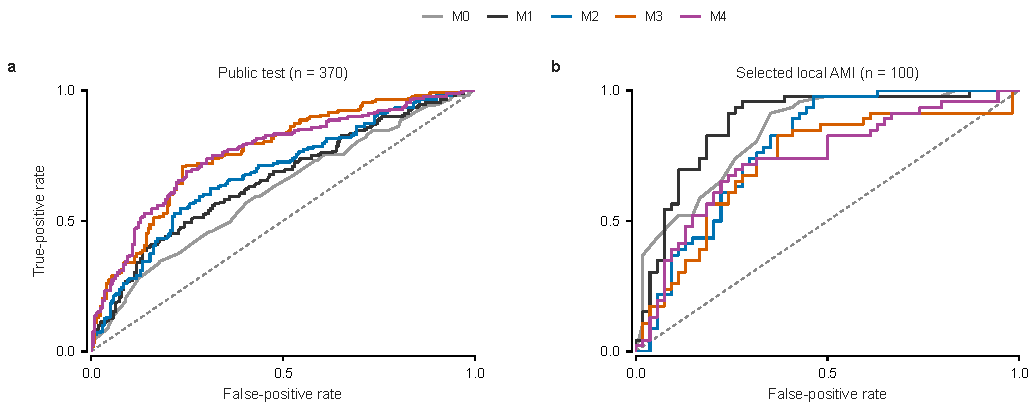
\includegraphics[width=\textwidth]{figures/FigureS1_ROC.pdf}\caption{Receiver operating characteristic curves for frozen models in the public test and selected local AMI cohorts.}\label{fig:s1}\end{figure}

\begin{figure}[!htbp]\centering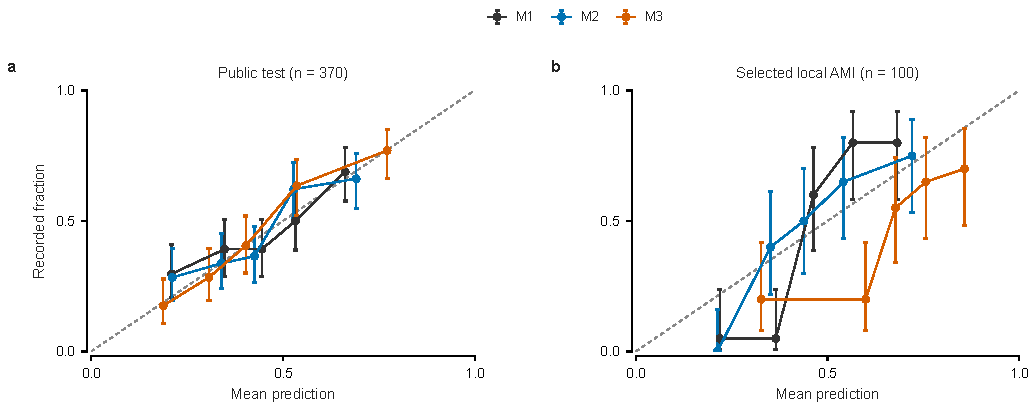
\includegraphics[width=\textwidth]{figures/FigureS2_calibration.pdf}\caption{Five-quantile calibration summaries for M1--M3 in both cohorts. Wilson intervals are pointwise, and risk bins are model specific.}\label{fig:s2}\end{figure}


\begin{figure}[!htbp]\centering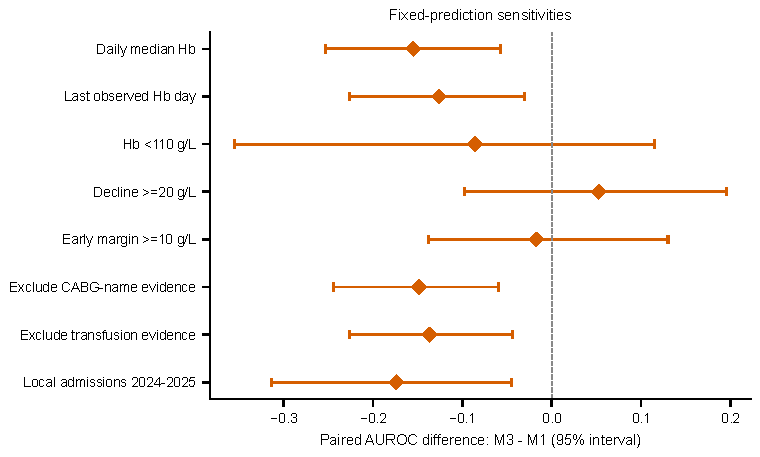
\includegraphics[width=\textwidth]{figures/FigureS3_sensitivity_increments.pdf}\caption{Paired M3-minus-M1 AUROC differences under alternative recorded outcomes and cohort restrictions. Bootstrap intervals condition on frozen models; outcome definitions were changed without model refitting.}\label{fig:s3}\end{figure}

\begin{figure}[!htbp]\centering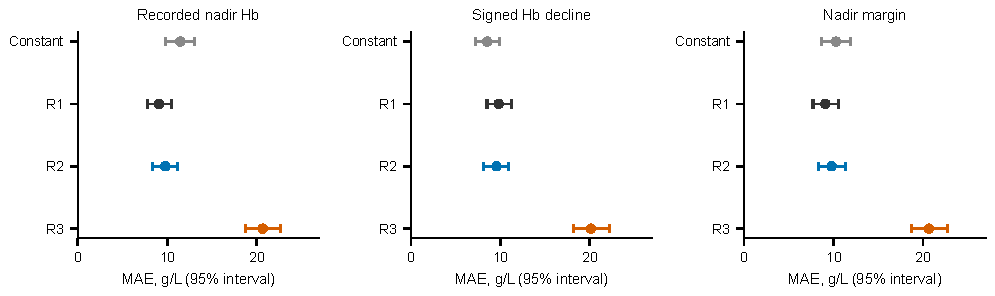
\includegraphics[width=\textwidth]{figures/FigureS4_continuous_outcomes.pdf}\caption{Mean absolute errors for continuous recorded-Hb outcomes under constant and frozen public Ridge models. All targets are conditional on future Hb observation; intervals use fixed-model bootstrap resampling.}\label{fig:s4}\end{figure}

\begin{figure}[!htbp]\centering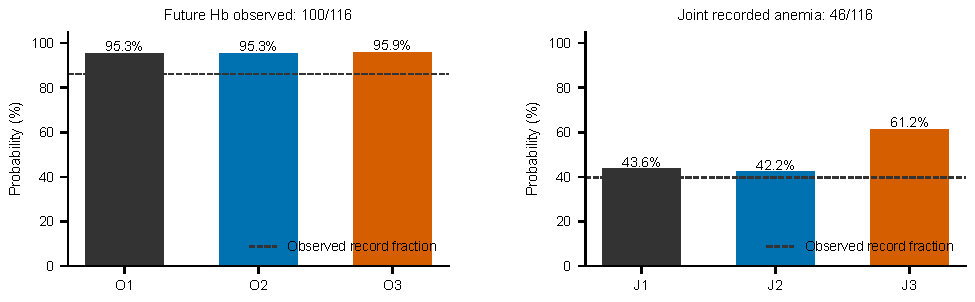
\includegraphics[width=\textwidth]{figures/FigureS5_observation_joint.pdf}\caption{Mean local frozen predictions for future Hb observation and joint recorded anemia (N=116). Dashed lines denote observed record fractions, not biological anemia incidence.}\label{fig:s5}\end{figure}
\clearpage
\begin{figure}[!htbp]\centering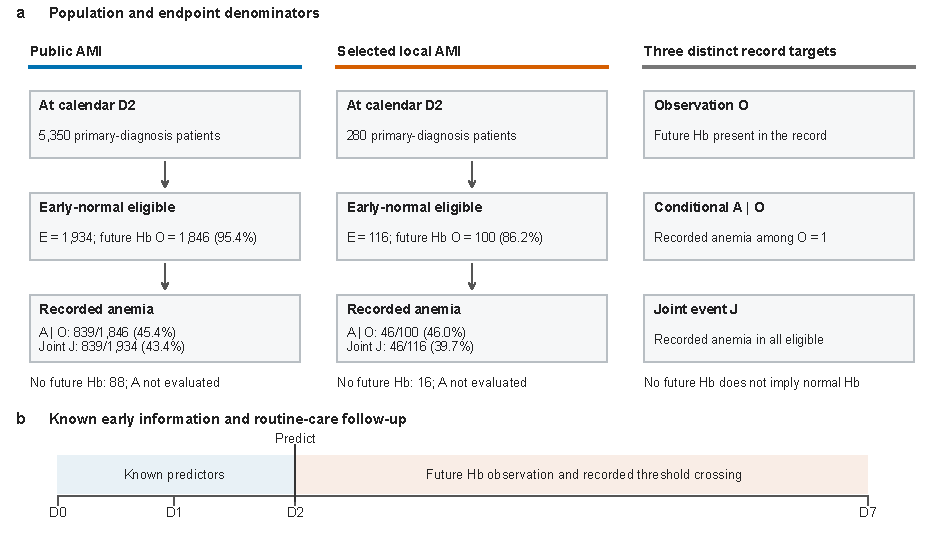
\includegraphics[width=\textwidth]{figures/Figure1_estimand_design.pdf}\caption{Population flow and outcome denominators for public and selected local AMI cohorts. Calendar-D0--1 predictors precede the D2 landmark; future Hb observation determines whether D2--7 conditional recorded anemia can be evaluated.}\label{fig:s6}\end{figure}
\end{document}